\providecommand{\devnum}[1]{#1}

\section{Experiments}
\label{sec:experiments}

The experiments are organised by the three questions of Section~\ref{sec:intro}. Question~1,
whether the cost of a job can be estimated before it runs, is answered in
Section~\ref{sec:prediction} and is not repeated here. This section takes the predictors as
given and asks what a scheduler should sort by (Section~\ref{sec:exp_rank}), what the per-job
guarantee costs and what it buys (Section~\ref{sec:exp_guard}), whether the bounds of
Section~\ref{sec:theory} hold on real traces (Section~\ref{sec:exp_bound}), and where the
method applies (Sections~\ref{sec:exp_cross} and~\ref{sec:exp_sens}).

\subsection{Setup}
\label{sec:exp_setup}

All scheduling runs replay the overlaid CodeBench pool built in
Section~\ref{sec:overlay}. The three load levels differ only in the pool size and the
five overlays only in the per-copy week shift, and every policy sees the same arrival
instants and the same service times, so the comparison is pathwise.
Table~\ref{tab:setup} collects the configuration and the selection protocol; the
metrics are defined in Section~\ref{sec:model} and the policy names in
Table~\ref{tab:policies}. We report the fraction of the FCFS-to-SJF gap closed and the
plain percentage reduction against FCFS side by side throughout, because they are
different numbers and the first is easy to read as the second.

\begin{table}[htbp]
\centering
\caption{Experimental configuration and the selection protocol for the guard parameters.}
\label{tab:setup}
\small
\begin{tabular}{p{0.24\textwidth}p{0.69\textwidth}}
\toprule
Item & Value \\
\midrule
Trace and pool & CodeBench development terms under the \devnum{60} s limit, overlaid as in Section~\ref{sec:overlay}; \devnum{17{,}634{,}760} jobs, \devnum{30} weeks, five overlays \\
Load levels & $k = \devnum{8/5/4}$ on four of the five overlays and $\devnum{7/5/4}$ on the fifth, whose work per busy hour is the lowest; busy-hour $\rho = \devnum{0.529} / \devnum{0.847} / \devnum{1.059}$ on overlay~0 \\
Single-server configuration & separate trace, \devnum{321} copies, \devnum{3{,}209{,}347} jobs, busy-hour $\rho = \devnum{0.80}$ at $k = 1$ \\
Primary metric & 99th percentile of the wait among jobs arriving in the \devnum{24}~h before their own deadline; secondary metrics as defined in Section~\ref{sec:model}, the gap closed printed beside the percentage reduction \\
Intervals & paired week-block bootstrap, \devnum{2{,}000} resamples of the \devnum{30} whole weeks, one draw of week multiplicities applied to every policy and to all five overlays \\
Promise to parameter & $B_{\max} = k(G - (3-2/k)L)$ with $L = \devnum{60}$ s, no data used \\
Budget shapes & one mechanism under one cap, three shapes: constant ($\gamma = \eta = 0$), age-relative ($+\,\eta k (t - a_q)$), queue-length ($+\,\gamma n_q$). Three pre-stated grids, \devnum{42} $+$ \devnum{162} $+$ \devnum{54} $=$ \devnum{258} points \\
Selection rule & a point is feasible if its harm is $\le G/2$ at each of the three load levels of each of the five validation overlays (\devnum{15} cells); the objective is the deadline-window gap closed in the worst cell; ties to smaller worst harm, then smaller $B_0$, then $\eta$, then $\gamma$. Guard($G$) is the winner over the three grids together; the winner inside each grid is an ablation row \\
Selected, $G = \devnum{300}$ s & age-relative: $B_0 = \devnum{60}k/4$ s, $\eta = \devnum{0.50}$, $\gamma = \devnum{0}$; worst-cell gap \devnum{0.4251}, worst-cell harm \devnum{122.8} s against a \devnum{150} s limit, \devnum{44} of \devnum{99} candidate points feasible \\
Selected, $G = \devnum{600}$ s & age-relative: $B_0 = \devnum{120}k/4$ s, $\eta = \devnum{0.75}$, $\gamma = \devnum{0}$; worst-cell gap \devnum{0.7216}, worst-cell harm \devnum{293.3} s against \devnum{300} s, \devnum{70} of \devnum{107} feasible \\
Selected, $G = \devnum{1200}$ s & queue-length: $B_0 = \devnum{0}$, $\eta = \devnum{0}$, $\gamma = \devnum{16}k/4$ s; worst-cell gap \devnum{0.7283}, worst-cell harm \devnum{145.3} s against \devnum{600} s, \devnum{95} of \devnum{111} feasible \\
Per-shape winners & constant: $B_0 = \devnum{329.671}$, \devnum{981.126}, \devnum{2{,}029.958}\,$k/4$ s at the three promises; age-relative: $(\devnum{60}, \devnum{0.50})$, $(\devnum{120}, \devnum{0.75})$, $(\devnum{360}, \devnum{0.75})$; queue-length: $\gamma = \devnum{16}k/4$ s with $B_0 = \devnum{0}$, \devnum{120}$k/4$ s, \devnum{0} \\
Comparators & As named in Table~\ref{tab:policies}. Fixed($G$) is the equal-promise budget $B_{\max}$, which the harm rule rejects at every promise; Skip($G$) takes the largest dispatch-charged count \eqref{eq:skip} allows at that $G$ and that cell's $k$ \\
\bottomrule
\end{tabular}
\end{table}
% Source of Table~\ref{tab:setup}: outputs/paper_tables/tab_setup.tex, produced by
%   `python scripts/emit_paper_tables.py` from outputs/dev_tables/ (see GENERATED.md for the
%   regeneration recipe and its check).  The trace, load-level, single-server, metric and
%   interval rows are unchanged from prechecks/main_v3/out_main_v31.txt section 2 (trace table,
%   rows primary 0-4 and k1) and are not produced by the package.  The grids, the rule, the
%   three selected points, the per-shape winners and the feasible counts are
%   protocol_lock.draft.json (search_grids.n_points 42/162/54, selection_rule, selected_parameters,
%   family_best) and docs/repo_build_status.md third pass, section 3.
%   Finite-skip count rule: \eqref{eq:skip}; per-cell counts in outputs/dev_tables/
%   policy_parameters.csv, column skip_count.

\subsection{What Was Selected on What}
\label{sec:exp_prov}

Three statements have to precede the numbers. First, the guard family and a coarse grid over
$(B_0, \eta)$ were explored on the evaluation trace before any validation-only selection
existed, so the selection reported above chooses inside a family that had already been narrowed
on the trace this section reports. Second, nothing here is held out. The validation pool is the
development terms minus the last one, which is held out of the selection and not of the
development process; the last development term on its own cannot load the pool, since it would
need \devnum{190} copies of its \devnum{8} class-terms, and it is therefore not evaluated
separately. We do not describe any figure in this section as out-of-sample, validated on test
data, or evidence of generalisation.

Third, every development number in this section comes from the released package: the
predictors are refitted deterministically from the recorded configuration, and the simulator
carries arrival instants, service times and budget arithmetic in exact integer microseconds, so
a rerun reproduces the tables byte for byte. Earlier exploratory runs of the same experiments
used a floating-point clock and a stored copy of the predictions; where both exist they agree
to the first decimal of a wait and differ in the second, and we print the package's values
throughout.

The three grids, the feasibility rule, the objective and the tie-break were fixed before the
grids were run, and the three shapes are searched at comparable density rather than one being
given a finer grid than the others. Two properties of the outcome are worth stating here rather
than in the discussion. The winning shape is not the same at every promise: the age-relative
shape wins the joint comparison at $G = \devnum{300}$ and $\devnum{600}$ s and the queue-length
shape at $G = \devnum{1200}$ s, where it reaches worst-cell gap \devnum{0.7283} at worst-cell
harm \devnum{145.3} s against \devnum{483.9} s for the best age-relative point. And the rule is
a worst-cell rule, so a single cell can decide it: dropping the one validation cell that decides
the $G = \devnum{600}$ choice moves that choice to $B_0 = \devnum{15}k/4$ s, $\eta =
\devnum{0.90}$, with worst-cell gap \devnum{0.7237}. Five overlays are five week-shifts of the
same class-terms and are not five independent tests. The sealed terms will be opened
once after the protocol freeze and reported in the same tables as an additional column, with the
parameters unchanged.
% Source of the paragraph above: protocol_lock.draft.json (grids, rule, selected points);
%   docs/repo_build_status.md third pass, sections 1 and 3 (the three grids at comparable
%   density, the nine family winners, the integer-microsecond kernel and the deterministic
%   refit); prechecks/main_v3/out_main_v32.txt section 4 (the drop-one-cell sensitivity table,
%   row G = 600 capped) and section 1 (what the second decimal of the older floating-point runs
%   does).

% SEALED-RESULTS-PLACEHOLDER

\subsection{Question 2: What to Rank By}
\label{sec:exp_rank}

Table~\ref{tab:rank} gives the unguarded policies at the three loads. Ranking by expected
cost is ahead of the log-scale score at the two higher loads and unresolved at the lightest:
the paired difference in gap closed is
\devnum{$-0.000$ $[-0.016, 0.013]$} at $\rho = \devnum{0.5}$,
\devnum{$+0.012$ $[0.004, 0.019]$} at $\rho = \devnum{0.8}$ and \devnum{$+0.019$ $[0.011,
0.024]$} at $\rho = \devnum{1.0}$. The control for refit noise, the same log-scale estimand
refitted from scratch, moves the gap by \devnum{$+0.001$ $[-0.002, 0.002]$},
\devnum{$-0.000$ $[-0.001, 0.001]$} and \devnum{$-0.000$ $[-0.001, 0.000]$}, so the advantage
is larger than the noise of refitting and is not produced by it; that control and the sequence
state come from the earlier development study and are the two rows of
Table~\ref{tab:rank} the package does not produce. The sequence state of
Section~\ref{sec:prediction} does not translate into a consistent gain and we do not claim it
as an improvement.

\begin{table}[htbp]
\centering
\caption{Unguarded policies, five overlays. Waits in seconds; gap and reduction on the
deadline-window p99, with \devnum{95\%} paired week-block intervals.}
\label{tab:rank}
\small
\setlength{\tabcolsep}{4pt}
\begin{tabular}{llrlrr}
\toprule
Load & Policy & p99$_{\mathrm{dl}}$ & Gap closed & Red.\ (\%) & Mean \\
\midrule
$\rho = \devnum{0.5}$, $k = \devnum{7.8}$
 & FCFS                 & \devnum{27.64} & \devnum{0.000} & \devnum{0.0} & \devnum{0.719} \\
 & SJF                  &\devnum{10.59} & \devnum{1.000} & \devnum{62.0 [58.7, 66.4]} & \devnum{0.228} \\
 & SPJF-log             &\devnum{14.71} & \devnum{0.754 [0.722, 0.777]} & \devnum{46.7 [43.9, 50.1]} & \devnum{0.296} \\
 & SPJF-log, refitted\textsuperscript{a}   &\devnum{14.72} & \devnum{0.753 [0.722, 0.776]} & \devnum{46.7 [44.0, 50.0]} & \devnum{0.295} \\
 & SPJF-E               &\devnum{14.68} & \devnum{0.754 [0.725, 0.776]} & \devnum{46.7 [43.9, 49.9]} & \devnum{0.292} \\
 & SPJF-E, GRU state\textsuperscript{a}    &\devnum{14.87} & \devnum{0.741 [0.707, 0.767]} & \devnum{45.9 [43.2, 48.8]} & \devnum{0.290} \\
\midrule
$\rho = \devnum{0.8}$, $k = \devnum{5}$
 & FCFS                 & \devnum{119.35} & \devnum{0.000} & \devnum{0.0} & \devnum{4.160} \\
 & SJF                  &\devnum{33.55} & \devnum{1.000} & \devnum{71.8 [67.0, 75.1]} & \devnum{0.959} \\
 & SPJF-log             &\devnum{44.36} & \devnum{0.873 [0.852, 0.887]} & \devnum{62.7 [57.5, 66.2]} & \devnum{1.252} \\
 & SPJF-log, refitted\textsuperscript{a}   &\devnum{44.41} & \devnum{0.873 [0.851, 0.886]} & \devnum{62.7 [57.4, 66.2]} & \devnum{1.251} \\
 & SPJF-E               &\devnum{43.33} & \devnum{0.885 [0.862, 0.899]} & \devnum{63.6 [58.1, 67.4]} & \devnum{1.232} \\
 & SPJF-E, GRU state\textsuperscript{a}    &\devnum{42.82} & \devnum{0.891 [0.870, 0.904]} & \devnum{64.0 [58.5, 67.7]} & \devnum{1.230} \\
\midrule
$\rho = \devnum{1.0}$, $k = \devnum{4}$
 & FCFS                 & \devnum{273.50} & \devnum{0.000} & \devnum{0.0} & \devnum{10.270} \\
 & SJF                  &\devnum{43.63} & \devnum{1.000} & \devnum{84.0 [79.6, 86.8]} & \devnum{1.696} \\
 & SPJF-log             &\devnum{67.17} & \devnum{0.897 [0.872, 0.914]} & \devnum{75.4 [70.2, 78.6]} & \devnum{2.354} \\
 & SPJF-log, refitted\textsuperscript{a}   &\devnum{67.36} & \devnum{0.896 [0.871, 0.913]} & \devnum{75.3 [70.1, 78.5]} & \devnum{2.352} \\
 & SPJF-E               &\devnum{62.79} & \devnum{0.916 [0.892, 0.930]} & \devnum{77.0 [71.6, 80.3]} & \devnum{2.294} \\
 & SPJF-E, GRU state\textsuperscript{a}    &\devnum{62.71} & \devnum{0.917 [0.895, 0.929]} & \devnum{77.0 [71.7, 80.3]} & \devnum{2.302} \\
\bottomrule
\end{tabular}

\vspace{2pt}
\begin{minipage}{\textwidth}
\footnotesize
\textsuperscript{a} These two rows are not produced by the released package, which fits only
the expected-cost and log-scale scores. They come from the earlier development study
(\texttt{prechecks/main\_v3}), which used a floating-point clock and a stored copy of the
predictions, and are printed at the values that study reported; the remaining rows differ from
it in the second decimal of a wait.
\end{minipage}
\end{table}
% Source of Table~\ref{tab:rank}: outputs/paper_tables/tab_rank.tex, produced by
%   `python scripts/emit_paper_tables.py` (see GENERATED.md), from
%   outputs/dev_tables/main_table.csv rows FCFS, SJF, SPJF-log, SPJF-E at levels 0, 1, 2;
%   columns p99_dl_s, gap_closed with gap_closed_lo/hi, reduction_pct with its interval, mean_s.
%   The gap intervals of FCFS and SJF are [0,0] and [1,1] by construction and are printed bare.
%   The paired differences quoted in the text are outputs/dev_tables/paired_differences.csv,
%   rows left = SPJF-E, right = SPJF-log at levels 0, 1, 2, columns difference_gap, gap_lo,
%   gap_hi.  The two footnote-a rows and the refit-noise control in the text are
%   prechecks/main_v3/out_main_v31.txt sections 4 and 5, rows SPJF-M4refit and SPJF-r1s.

Scores other than a conditional mean were fitted on the same features and run through the same
simulator (Table~\ref{tab:scores}). A predicted quantile loses at every load, and the loss grows
as the quantile falls, which is what a scheduler that needs an additive quantity rather than a
threshold should do; squared error on raw seconds also loses at every load, so it is the change
of estimand and not the change of scale that produces the difference. A two-class rule that
sends predicted-heavy jobs behind predicted-light ones and runs FCFS inside each class reaches a
deadline-window p99 of \devnum{64.05} s at $\rho = \devnum{0.8}$ on the first overlay, against
\devnum{43.86} s for the full ordering on the same overlay, so most of the benefit comes from
the fine ordering inside the light class rather than from separating the two classes.

\begin{table}[htbp]
\centering
\caption{Ranking scores fitted on one feature set and run through one simulator: fraction of the
deadline-window gap closed, five overlays, and the paired difference against the log-scale
score.}
\label{tab:scores}
\small
\begin{tabular}{lcccc}
\toprule
Score & $\rho = \devnum{0.5}$ & $\rho = \devnum{0.8}$ & $\rho = \devnum{1.0}$ & Difference at $\rho = \devnum{1.0}$ \\
\midrule
SPJF-log                   & \devnum{0.7528} & \devnum{0.8728} & \devnum{0.8967} & --- \\
SPJF-E                     & \devnum{0.7515} & \devnum{0.8847} & \devnum{0.9159} & \devnum{$+0.0191$ $[+0.0111, +0.0238]$} \\
Expected cost, gamma hurdle & \devnum{0.7404} & \devnum{0.8826} & \devnum{0.9141} & \devnum{$+0.0174$ $[+0.0082, +0.0223]$} \\
Probability of heavy       & \devnum{0.7476} & \devnum{0.8821} & \devnum{0.9122} & \devnum{$+0.0155$ $[+0.0066, +0.0199]$} \\
Predicted 99th percentile  & \devnum{0.7245} & \devnum{0.8742} & \devnum{0.9005} & \devnum{$+0.0038$ $[-0.0050, +0.0097]$} \\
Predicted 90th percentile  & \devnum{0.7024} & \devnum{0.8470} & \devnum{0.8755} & \devnum{$-0.0212$ $[-0.0297, -0.0156]$} \\
Predicted median           & \devnum{0.7071} & \devnum{0.8196} & \devnum{0.8402} & \devnum{$-0.0565$ $[-0.0684, -0.0463]$} \\
Squared error, raw seconds & \devnum{0.7197} & \devnum{0.8585} & \devnum{0.8873} & \devnum{$-0.0094$ $[-0.0194, -0.0043]$} \\
\bottomrule
\end{tabular}
\end{table}
% Source of Table~\ref{tab:scores}: prechecks/ranking_score/out_table_primary_5reps.txt, the
%   three blocks "primary, reps 0,1,2,3,4, busy-hour rho target 0.5 / 0.8 / 1.0"; column
%   gain_p99dl for the three load columns and column dgain_p99dl_vs_M4 of the rho 1.0 block for
%   the last column.  Rows SPJF-M4 / SPJF-tweedie / SPJF-hurdle / SPJF-phv / SPJF-q99 /
%   SPJF-q90 / SPJF-q50 / SPJF-l2raw.  This is a separate study with its own fits, which is why
%   its M4 and Tweedie figures differ in the third decimal from Table~\ref{tab:rank}.
%   Two-class figures in the text: prechecks/ranking_score/out_sim_primary_rep0_twoclass.txt,
%   block primary_rep0_r0.8_twoclass, rows 2CLASS-FCFS-tau0.02 and SPJF-tweedie, column w_p99_dl.

The two kinds of error do not cost the same. Replacing the largest \devnum{1\%} of
underestimates by the true cost, and leaving the rest of the score alone, moves the
deadline-window p99 at $\rho = \devnum{1.0}$ from \devnum{66.57} s to \devnum{45.01} s on the
first overlay and from \devnum{65.02} s to \devnum{45.32} s on the second, which is
\devnum{0.91} of the distance to the SJF reference in both. Repairing the largest
\devnum{1\%} of overestimates instead moves it to \devnum{60.37} s and \devnum{59.72} s, which
is \devnum{0.26} and \devnum{0.24} of that distance. At \devnum{0.1\%} the two figures are
\devnum{0.47} and \devnum{0.04}. Treating a heavy job as light and letting it run first is the
expensive mistake, by about an order of magnitude, which is the argument of
Section~\ref{sec:rank} for fitting an estimand rather than minimising a symmetric loss.
% Source of the asymmetry figures: prechecks/ranking_score/out_sim_primary_rep0_mech.txt and
%   out_sim_primary_rep1_mech.txt, blocks primary_rep{0,1}_r1_mech, column w_p99_dl, rows
%   SPJF-M4, SJF-ref, ORACLE-top1.0pct-under, ORACLE-top1.0pct-over, ORACLE-top0.1pct-under,
%   ORACLE-top0.1pct-over.  The fractions are (SPJF-M4 - ORACLE)/(SPJF-M4 - SJF-ref) per
%   overlay: 0.9099 / 0.9099 (under 1%), 0.2619 / 0.2448 (over 1%), 0.4882 / 0.4495 (under
%   0.1%), 0.0509 / 0.0320 (over 0.1%).

\subsection{Question 3: What the Guarantee Costs and Buys}
\label{sec:exp_guard}

Table~\ref{tab:guard} reports the guarded policies at three promises and three loads, and
Figure~\ref{fig:gapvsg} plots the gap closed against the promise. The cost of the promise
depends on the promise and on the load. At $\rho = \devnum{1.0}$, Guard($\devnum{600}$) closes
\devnum{0.801} of the FCFS-to-SJF gap against \devnum{0.916} for the unguarded policy, so it
gives up \devnum{0.115} of the gap at a promise of ten job-limits, about an eighth of what the
unguarded ordering buys; at $G = \devnum{1200}$ s the cost is \devnum{0.087} and at
$G = \devnum{300}$ s, five job-limits, \devnum{0.438}. These three are differences of the point
values in Table~\ref{tab:guard}; the package's paired intervals are computed between guarded
policies, which is where the comparisons below sit.

% Wider than the MDPI text block: set across the full page with the template's
% adjustwidth/\extralength mechanism.
\begin{table}[htbp]
\begin{adjustwidth}{-\extralength}{0cm}
\centering
\caption{The guard at three promises, its three budget shapes, and the comparators. Guard($G$)
is the shape the selection rule picks over all three grids; Guard-fixed, Guard-age and
Guard-queue are the winners inside the constant, age-relative and queue-length grid, so one of
them repeats Guard($G$) at each promise. Fixed($G$) spends the whole cap at the same promise and
is infeasible under the harm rule. Budgets scale as $k/4$ and the skip count is the largest
integer with $(N + 2k-2)L/k \le G$, so both differ with the cell's $k$: at
$\rho = \devnum{0.5}$ the four overlays at $k = \devnum{8}$ run $N = \devnum{26}/\devnum{66}/\devnum{146}$
and the fifth, at $k = \devnum{7}$, runs $\devnum{23}/\devnum{58}/\devnum{128}$, which is what
the column prints. Excess, harm and worst heavy wait are the worst over the five overlays, the
rest are means.}
\label{tab:guard}
\small
\setlength{\tabcolsep}{3pt}
\begin{tabular}{llrrlrrrr}
\toprule
Load & Policy & Promise & p99$_{\mathrm{dl}}$ & Gap closed & Red.\ (\%) & Max exc. & Harm & Fired (\%) \\
\midrule
\multicolumn{9}{l}{$\rho = \devnum{0.5}$, $k = \devnum{7.8}$; FCFS p99$_{\mathrm{dl}} = \devnum{27.64}$ s, SPJF-E \devnum{14.68} s with max excess \devnum{1{,}241.4} s} \\
 & Guard($\devnum{300}$)      & \devnum{300} & \devnum{15.58} & \devnum{0.705 [0.678, 0.724]} & \devnum{43.7} & \devnum{192.5} & \devnum{132.1} & \devnum{1.35} \\
 & Guard-fixed($\devnum{300}$) & \devnum{300} & \devnum{15.75} & \devnum{0.697 [0.673, 0.717]} & \devnum{43.2} & \devnum{143.0} & \devnum{132.1} & \devnum{2.12} \\
 & Guard-age($\devnum{300}$)  & \devnum{300} & \devnum{15.58} & \devnum{0.705 [0.678, 0.724]} & \devnum{43.7} & \devnum{192.5} & \devnum{132.1} & \devnum{1.35} \\
 & Guard-queue($\devnum{300}$) & \devnum{300} & \devnum{15.27} & \devnum{0.723 [0.697, 0.742]} & \devnum{44.8} & \devnum{193.4} & \devnum{94.3} & \devnum{21.60} \\
 & Fixed($\devnum{300}$)      & \devnum{300} & \devnum{15.30} & \devnum{0.721 [0.696, 0.738]} & \devnum{44.7} & \devnum{193.0} & \devnum{181.8} & \devnum{0.77} \\
 & Skip($\devnum{300}$), $N=23$ & \devnum{300} & \devnum{26.38} & \devnum{0.078 [0.052, 0.107]} & \devnum{4.8} & \devnum{62.1} & \devnum{59.6} & \devnum{45.41} \\
 & Guard($\devnum{600}$)      & \devnum{600} & \devnum{14.97} & \devnum{0.740 [0.713, 0.760]} & \devnum{45.8} & \devnum{492.2} & \devnum{237.0} & \devnum{0.17} \\
 & Guard-fixed($\devnum{600}$) & \devnum{600} & \devnum{15.09} & \devnum{0.733 [0.706, 0.752]} & \devnum{45.4} & \devnum{298.7} & \devnum{237.0} & \devnum{0.36} \\
 & Guard-age($\devnum{600}$)  & \devnum{600} & \devnum{14.97} & \devnum{0.740 [0.713, 0.760]} & \devnum{45.8} & \devnum{492.2} & \devnum{237.0} & \devnum{0.17} \\
 & Guard-queue($\devnum{600}$) & \devnum{600} & \devnum{14.88} & \devnum{0.744 [0.718, 0.765]} & \devnum{46.1} & \devnum{504.5} & \devnum{106.0} & \devnum{0.16} \\
 & Fixed($\devnum{600}$)      & \devnum{600} & \devnum{14.91} & \devnum{0.742 [0.715, 0.763]} & \devnum{46.0} & \devnum{493.3} & \devnum{237.0} & \devnum{0.11} \\
 & Skip($\devnum{600}$), $N=58$ & \devnum{600} & \devnum{24.64} & \devnum{0.184 [0.135, 0.233]} & \devnum{11.5} & \devnum{100.2} & \devnum{63.3} & \devnum{37.26} \\
 & Guard($\devnum{1200}$)     & \devnum{1200} & \devnum{14.84} & \devnum{0.746 [0.719, 0.768]} & \devnum{46.2} & \devnum{907.8} & \devnum{94.3} & \devnum{22.01} \\
 & Guard-fixed($\devnum{1200}$) & \devnum{1200} & \devnum{14.83} & \devnum{0.747 [0.719, 0.768]} & \devnum{46.2} & \devnum{557.8} & \devnum{237.0} & \devnum{0.06} \\
 & Guard-age($\devnum{1200}$) & \devnum{1200} & \devnum{14.73} & \devnum{0.751 [0.723, 0.773]} & \devnum{46.5} & \devnum{1{,}049.1} & \devnum{237.0} & \devnum{0.01} \\
 & Guard-queue($\devnum{1200}$) & \devnum{1200} & \devnum{14.84} & \devnum{0.746 [0.719, 0.768]} & \devnum{46.2} & \devnum{907.8} & \devnum{94.3} & \devnum{22.01} \\
 & Fixed($\devnum{1200}$)     & \devnum{1200} & \devnum{14.70} & \devnum{0.753 [0.724, 0.775]} & \devnum{46.6} & \devnum{1{,}077.0} & \devnum{237.0} & \devnum{0.00} \\
 & Skip($\devnum{1200}$), $N=128$ & \devnum{1200} & \devnum{21.62} & \devnum{0.367 [0.288, 0.432]} & \devnum{22.8} & \devnum{102.3} & \devnum{67.6} & \devnum{28.80} \\
\midrule
\multicolumn{9}{l}{$\rho = \devnum{0.8}$, $k = \devnum{5}$; FCFS p99$_{\mathrm{dl}} = \devnum{119.35}$ s, SPJF-E \devnum{43.33} s with max excess \devnum{3{,}044.5} s} \\
 & Guard($\devnum{300}$)      & \devnum{300} & \devnum{55.94} & \devnum{0.738 [0.697, 0.761]} & \devnum{53.0} & \devnum{209.7} & \devnum{114.1} & \devnum{11.57} \\
 & Guard-fixed($\devnum{300}$) & \devnum{300} & \devnum{64.44} & \devnum{0.640 [0.543, 0.699]} & \devnum{45.9} & \devnum{171.6} & \devnum{151.1} & \devnum{20.62} \\
 & Guard-age($\devnum{300}$)  & \devnum{300} & \devnum{55.94} & \devnum{0.738 [0.697, 0.761]} & \devnum{53.0} & \devnum{209.7} & \devnum{114.1} & \devnum{11.57} \\
 & Guard-queue($\devnum{300}$) & \devnum{300} & \devnum{54.69} & \devnum{0.753 [0.713, 0.777]} & \devnum{54.0} & \devnum{210.7} & \devnum{117.6} & \devnum{17.53} \\
 & Fixed($\devnum{300}$)      & \devnum{300} & \devnum{53.83} & \devnum{0.763 [0.721, 0.785]} & \devnum{54.8} & \devnum{210.9} & \devnum{195.4} & \devnum{10.75} \\
 & Skip($\devnum{300}$), $N=17$ & \devnum{300} & \devnum{119.20} & \devnum{0.002 [-0.001, 0.009]} & \devnum{0.1} & \devnum{64.2} & \devnum{58.8} & \devnum{80.53} \\
 & Guard($\devnum{600}$)      & \devnum{600} & \devnum{47.47} & \devnum{0.837 [0.815, 0.851]} & \devnum{60.1} & \devnum{507.8} & \devnum{319.6} & \devnum{1.31} \\
 & Guard-fixed($\devnum{600}$) & \devnum{600} & \devnum{49.85} & \devnum{0.809 [0.786, 0.824]} & \devnum{58.1} & \devnum{315.4} & \devnum{285.7} & \devnum{4.72} \\
 & Guard-age($\devnum{600}$)  & \devnum{600} & \devnum{47.47} & \devnum{0.837 [0.815, 0.851]} & \devnum{60.1} & \devnum{507.8} & \devnum{319.6} & \devnum{1.31} \\
 & Guard-queue($\devnum{600}$) & \devnum{600} & \devnum{47.69} & \devnum{0.834 [0.814, 0.847]} & \devnum{59.9} & \devnum{508.5} & \devnum{117.7} & \devnum{1.35} \\
 & Fixed($\devnum{600}$)      & \devnum{600} & \devnum{47.03} & \devnum{0.842 [0.824, 0.853]} & \devnum{60.5} & \devnum{502.6} & \devnum{447.1} & \devnum{1.16} \\
 & Skip($\devnum{600}$), $N=42$ & \devnum{600} & \devnum{118.69} & \devnum{0.008 [-0.002, 0.026]} & \devnum{0.6} & \devnum{97.5} & \devnum{63.5} & \devnum{74.02} \\
 & Guard($\devnum{1200}$)     & \devnum{1200} & \devnum{46.85} & \devnum{0.844 [0.823, 0.857]} & \devnum{60.6} & \devnum{1{,}104.9} & \devnum{117.6} & \devnum{9.93} \\
 & Guard-fixed($\devnum{1200}$) & \devnum{1200} & \devnum{46.76} & \devnum{0.845 [0.826, 0.857]} & \devnum{60.7} & \devnum{581.8} & \devnum{469.2} & \devnum{0.86} \\
 & Guard-age($\devnum{1200}$) & \devnum{1200} & \devnum{45.16} & \devnum{0.864 [0.844, 0.876]} & \devnum{62.0} & \devnum{1{,}102.9} & \devnum{370.5} & \devnum{0.29} \\
 & Guard-queue($\devnum{1200}$) & \devnum{1200} & \devnum{46.85} & \devnum{0.844 [0.823, 0.857]} & \devnum{60.6} & \devnum{1{,}104.9} & \devnum{117.6} & \devnum{9.93} \\
 & Fixed($\devnum{1200}$)     & \devnum{1200} & \devnum{45.32} & \devnum{0.862 [0.842, 0.874]} & \devnum{61.9} & \devnum{1{,}106.3} & \devnum{469.2} & \devnum{0.22} \\
 & Skip($\devnum{1200}$), $N=92$ & \devnum{1200} & \devnum{117.48} & \devnum{0.022 [0.004, 0.074]} & \devnum{1.6} & \devnum{162.5} & \devnum{83.6} & \devnum{66.10} \\
\midrule
\multicolumn{9}{l}{$\rho = \devnum{1.0}$, $k = \devnum{4}$; FCFS p99$_{\mathrm{dl}} = \devnum{273.50}$ s, SPJF-E \devnum{62.79} s with max excess \devnum{5{,}904.5} s} \\
 & Guard($\devnum{300}$)      & \devnum{300} & \devnum{163.40} & \devnum{0.478 [0.387, 0.602]} & \devnum{40.2} & \devnum{229.1} & \devnum{134.8} & \devnum{28.64} \\
 & Guard-fixed($\devnum{300}$) & \devnum{300} & \devnum{223.69} & \devnum{0.217 [0.151, 0.359]} & \devnum{18.2} & \devnum{165.1} & \devnum{158.4} & \devnum{41.50} \\
 & Guard-age($\devnum{300}$)  & \devnum{300} & \devnum{163.40} & \devnum{0.478 [0.387, 0.602]} & \devnum{40.2} & \devnum{229.1} & \devnum{134.8} & \devnum{28.64} \\
 & Guard-queue($\devnum{300}$) & \devnum{300} & \devnum{169.22} & \devnum{0.453 [0.368, 0.607]} & \devnum{38.1} & \devnum{231.4} & \devnum{144.8} & \devnum{30.99} \\
 & Fixed($\devnum{300}$)      & \devnum{300} & \devnum{169.29} & \devnum{0.453 [0.369, 0.619]} & \devnum{38.1} & \devnum{222.6} & \devnum{208.2} & \devnum{28.33} \\
 & Skip($\devnum{300}$), $N=14$ & \devnum{300} & \devnum{273.14} & \devnum{0.001 [-0.001, 0.003]} & \devnum{0.1} & \devnum{81.3} & \devnum{81.3} & \devnum{90.36} \\
 & Guard($\devnum{600}$)      & \devnum{600} & \devnum{89.24} & \devnum{0.801 [0.764, 0.842]} & \devnum{67.3} & \devnum{523.7} & \devnum{339.9} & \devnum{7.15} \\
 & Guard-fixed($\devnum{600}$) & \devnum{600} & \devnum{116.75} & \devnum{0.682 [0.601, 0.764]} & \devnum{57.3} & \devnum{325.4} & \devnum{292.9} & \devnum{17.50} \\
 & Guard-age($\devnum{600}$)  & \devnum{600} & \devnum{89.24} & \devnum{0.801 [0.764, 0.842]} & \devnum{67.3} & \devnum{523.7} & \devnum{339.9} & \devnum{7.15} \\
 & Guard-queue($\devnum{600}$) & \devnum{600} & \devnum{91.09} & \devnum{0.793 [0.758, 0.833]} & \devnum{66.6} & \devnum{515.8} & \devnum{123.4} & \devnum{7.08} \\
 & Fixed($\devnum{600}$)      & \devnum{600} & \devnum{86.53} & \devnum{0.813 [0.778, 0.851]} & \devnum{68.3} & \devnum{515.8} & \devnum{465.5} & \devnum{7.23} \\
 & Skip($\devnum{600}$), $N=34$ & \devnum{600} & \devnum{272.98} & \devnum{0.002 [-0.004, 0.006]} & \devnum{0.2} & \devnum{112.4} & \devnum{82.4} & \devnum{86.25} \\
 & Guard($\devnum{1200}$)     & \devnum{1200} & \devnum{82.67} & \devnum{0.830 [0.801, 0.857]} & \devnum{69.7} & \devnum{1{,}110.4} & \devnum{144.8} & \devnum{6.21} \\
 & Guard-fixed($\devnum{1200}$) & \devnum{1200} & \devnum{83.32} & \devnum{0.827 [0.798, 0.860]} & \devnum{69.5} & \devnum{576.5} & \devnum{522.7} & \devnum{5.76} \\
 & Guard-age($\devnum{1200}$) & \devnum{1200} & \devnum{72.52} & \devnum{0.874 [0.851, 0.893]} & \devnum{73.4} & \devnum{1{,}117.3} & \devnum{453.3} & \devnum{0.81} \\
 & Guard-queue($\devnum{1200}$) & \devnum{1200} & \devnum{82.67} & \devnum{0.830 [0.801, 0.857]} & \devnum{69.7} & \devnum{1{,}110.4} & \devnum{144.8} & \devnum{6.21} \\
 & Fixed($\devnum{1200}$)     & \devnum{1200} & \devnum{72.94} & \devnum{0.872 [0.846, 0.893]} & \devnum{73.3} & \devnum{1{,}112.9} & \devnum{708.8} & \devnum{0.73} \\
 & Skip($\devnum{1200}$), $N=74$ & \devnum{1200} & \devnum{273.08} & \devnum{0.002 [-0.009, 0.013]} & \devnum{0.1} & \devnum{169.7} & \devnum{105.0} & \devnum{80.69} \\
\bottomrule
\end{tabular}
\end{adjustwidth}
\end{table}
% Source of Table~\ref{tab:guard}: outputs/paper_tables/tab_guard.tex, produced by
%   `python scripts/emit_paper_tables.py` (see GENERATED.md), from
%   outputs/dev_tables/main_table.csv, rows Guard / Guard-fixed / Guard-age / Guard-queue /
%   Fixed / Skip at each promise and levels 0, 1, 2; columns p99_dl_s, gap_closed with
%   gap_closed_lo/hi, reduction_pct, max_excess_s, harm_s, fired_pct.  Block headers are the
%   FCFS and SPJF-E rows of the same file.  The promise column is G; the skip counts come from
%   outputs/dev_tables/policy_parameters.csv, column skip_count, which is per cell, so the
%   rho = 0.5 block carries two values and the caption prints both (verifier item G3).
%   The "Fixed, admitted" rows of the previous version are gone: the fixed shape is now searched
%   on its own pre-stated grid and appears as Guard-fixed(G) at the full promise.

% Figure: gap closed against the promised excess G, for the joint winner, the
% constant-shape ablation and the two comparators, at the three load levels.
% Every coordinate below is a cell of Table~\ref{tab:guard} (column "Gap closed",
% rows Guard(G) / Guard-fixed(G) / Fixed(G) / Skip(G) at G = 300, 600, 1200 s),
% which comes from outputs/paper_tables/tab_guard.tex.  No new computation.
\begin{figure}[htbp]
\centering
\resizebox{\textwidth}{!}{%
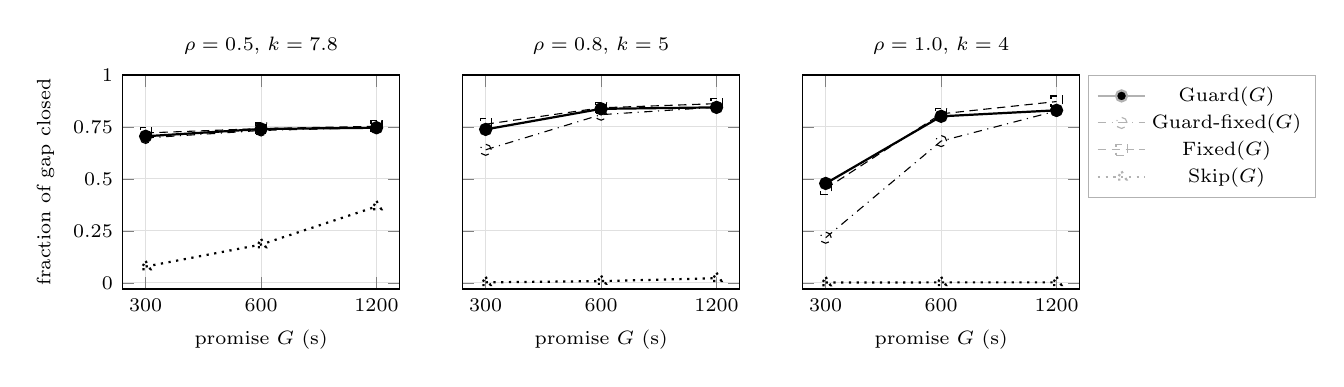
\begin{tikzpicture}[font=\footnotesize]
\pgfplotsset{
  gapaxis/.style={
    width=5.1cm, height=4.3cm,
    symbolic x coords={300,600,1200}, xtick=data,
    xlabel={promise $G$ (s)}, ymin=-0.03, ymax=1.0,
    ytick={0,0.25,0.5,0.75,1}, grid=major, grid style={black!12},
    tick label style={font=\scriptsize}, label style={font=\scriptsize},
    title style={font=\scriptsize, yshift=-2pt},
  },
}
\begin{axis}[gapaxis, ylabel={fraction of gap closed},
             title={$\rho = 0.5$, $k = 7.8$}, name=p1]
  \addplot[mark=*,thick]            coordinates {(300,0.705) (600,0.740) (1200,0.746)};
  \addplot[mark=o,dash dot]         coordinates {(300,0.697) (600,0.733) (1200,0.747)};
  \addplot[mark=square,densely dashed] coordinates {(300,0.721) (600,0.742) (1200,0.753)};
  \addplot[mark=triangle,dotted,thick] coordinates {(300,0.078) (600,0.184) (1200,0.367)};
\end{axis}
\begin{axis}[gapaxis, title={$\rho = 0.8$, $k = 5$},
             at={(p1.east)}, anchor=west, xshift=8mm, name=p2, yticklabels={}]
  \addplot[mark=*,thick]            coordinates {(300,0.738) (600,0.837) (1200,0.844)};
  \addplot[mark=o,dash dot]         coordinates {(300,0.640) (600,0.809) (1200,0.845)};
  \addplot[mark=square,densely dashed] coordinates {(300,0.763) (600,0.842) (1200,0.862)};
  \addplot[mark=triangle,dotted,thick] coordinates {(300,0.002) (600,0.008) (1200,0.022)};
\end{axis}
\begin{axis}[gapaxis, title={$\rho = 1.0$, $k = 4$},
             at={(p2.east)}, anchor=west, xshift=8mm, yticklabels={},
             legend style={font=\scriptsize, at={(1.03,1.0)}, anchor=north west,
                           draw=black!30, row sep=-1pt}]
  \addplot[mark=*,thick]            coordinates {(300,0.478) (600,0.801) (1200,0.830)};
  \addlegendentry{Guard($G$)}
  \addplot[mark=o,dash dot]         coordinates {(300,0.217) (600,0.682) (1200,0.827)};
  \addlegendentry{Guard-fixed($G$)}
  \addplot[mark=square,densely dashed] coordinates {(300,0.453) (600,0.813) (1200,0.872)};
  \addlegendentry{Fixed($G$)}
  \addplot[mark=triangle,dotted,thick] coordinates {(300,0.001) (600,0.002) (1200,0.002)};
  \addlegendentry{Skip($G$)}
\end{axis}
\end{tikzpicture}}
\caption{Original source-clock scores (optimistic reference): what each budget shape keeps of the FCFS-to-SJF gap as the promised
excess $G$ is relaxed. Every point is a ``Gap closed'' cell of
Table~\ref{tab:guard}; the intervals are in that table and are omitted here.
All four policies carry the same promise at a given $G$, since the promise
depends on the cap alone. The gap between Guard($G$) and its constant-shape
ablation opens where the promise is tight and the load is high and closes
elsewhere; counting positions rather than work (Skip) collapses at the two higher
loads; Fixed($G$), which spends the whole cap, buys its gap with harm the
selection rule rejects.}
\label{fig:gapvsg}
\end{figure}


\paragraph{What the shape of the budget is worth.}
The promise is the cap's alone, so the three shapes are compared at a fixed promise and the
question is only how much of the base policy's benefit each keeps and who pays for it. The
shape matters where the promise is tight and the load is high, and hardly at all elsewhere. At
$G = \devnum{600}$ s the constant shape trails the joint winner by
\devnum{0.007 [0.003, 0.012]}, \devnum{0.028 [0.020, 0.038]} and \devnum{0.119 [0.074, 0.176]}
of the gap as the load rises through the three levels, each interval clear of zero; at
$G = \devnum{300}$ s the same three differences are \devnum{0.008 [-0.002, 0.015]},
\devnum{0.099 [0.056, 0.157]} and \devnum{0.262 [0.202, 0.288]}; and at $G = \devnum{1200}$ s
they are \devnum{$-0.001$}, \devnum{$-0.001$} and \devnum{0.003}, none of the three intervals
excluding zero. At a loose promise and a light load the shape is not doing measurable work.

The other axis is harm. At $G = \devnum{600}$ s the queue-length shape reaches within
\devnum{0.008} of the joint winner's gap at every load while its worst-overlay harm is
\devnum{106.0}, \devnum{117.7} and \devnum{123.4} s against the winner's \devnum{237.0},
\devnum{319.6} and \devnum{339.9} s, under half at every load. That is also why
the rule picks the queue-length shape at $G = \devnum{1200}$ s, where the three shapes are
within \devnum{0.005} of one another on the validation objective and it has the smallest worst
harm. A shape moves where the promise is spent more than it moves how much is kept.

Fixed($G$), which spends the whole cap, is reported for reference and is not a candidate: its
worst-overlay harm is \devnum{181.8}, \devnum{195.4} and \devnum{208.2} s at
$G = \devnum{300}$ s against a \devnum{150} s limit, \devnum{237.0}, \devnum{447.1} and
\devnum{465.5} s at $G = \devnum{600}$ s against \devnum{300} s, and \devnum{237.0},
\devnum{469.2} and \devnum{708.8} s at $G = \devnum{1200}$ s against \devnum{600} s, so the
selection rule rejects it at all three promises. It is also ahead of the joint winner on the gap
closed in eight of the nine cells, by up to \devnum{0.042}, which is what buying gap with harm
looks like; we make no claim that any shape beats it on the gap at equal promise.
% Source of the two paragraphs above: outputs/dev_tables/paired_differences.csv (rows
%   left = Guard(G), right = Guard-fixed(G) / Guard-queue(G) at levels 0, 1, 2; columns
%   difference_gap, gap_lo, gap_hi, excludes_zero_gap) and the Harm and Gap-closed columns of
%   Table~\ref{tab:guard}.  The worst-cell validation objectives of the three shapes at
%   G = 1200 s (0.7257 / 0.7273 / 0.7283) are docs/repo_build_status.md third pass, section 3.

Counting positions rather than work buys almost nothing on this load
(Figure~\ref{fig:gapvsg}, dotted). The reason is in the cost distribution rather than in the
mechanism: overtakers on this trace are overwhelmingly shorter than a second, so a count sized
for the worst case $N L$ is exhausted long before the work it permits is, and the baseline
forces most dispatches back to the queue head. It is charged at dispatch and given the largest
count \eqref{eq:skip} allows at each promise, \devnum{34} rather than \devnum{30} passes at
$k = \devnum{4}$ and $G = \devnum{600}$ s; charging at completion instead changes the gap closed
by at most \devnum{0.015}, and by at most \devnum{0.001} at the two higher loads.

Corrupted scores separate what the guard does from what it does not do
(Table~\ref{tab:adv}, Figure~\ref{fig:excess}). Under a reversed order, a random order, or a
score that calls the truly longest \devnum{1\%} the shortest, the unguarded policy delays some
job by more than \devnum{6{,}000} s beyond FCFS at full load, and Guard($\devnum{600}$) holds
every job inside its promise. The deadline-window p99 is not rescued: it stays at
\devnum{546.5}, \devnum{261.9} and \devnum{543.6} s against \devnum{273.50} s for FCFS, which is
worse than FCFS for two of the three. This is the guarantee behaving as stated. It is per job
and additive, so a guarded run may have a worse quantile than FCFS, by at most $G$, and what it
removes is the worst single job rather than the shape of the tail.

\begin{table}[htbp]
\centering
\caption{Deliberately corrupted scores, unguarded and under Guard($\devnum{600}$).
Waits and excesses in seconds.}
\label{tab:adv}
\small
\begin{tabular}{llrrrrr}
\toprule
 & & \multicolumn{2}{c}{p99$_{\mathrm{dl}}$} & \multicolumn{2}{c}{Max excess} & Harm \\
Load & Score & unguarded & guarded & unguarded & guarded & guarded \\
\midrule
$\rho = \devnum{0.5}$ & reversed    & \devnum{42.72}  & \devnum{43.39}  & \devnum{1{,}240.1} & \devnum{497.1} & \devnum{287.1} \\
                      & random      & \devnum{16.82}  & \devnum{17.12}  & \devnum{1{,}307.7} & \devnum{489.9} & \devnum{324.0} \\
                      & longest as shortest & \devnum{38.24} & \devnum{38.71} & \devnum{1{,}305.8} & \devnum{497.1} & \devnum{273.4} \\
$\rho = \devnum{0.8}$ & reversed    & \devnum{228.12} & \devnum{232.41} & \devnum{3{,}387.9} & \devnum{513.5} & \devnum{323.4} \\
                      & random      & \devnum{78.52}  & \devnum{88.39}  & \devnum{3{,}319.4} & \devnum{504.5} & \devnum{352.3} \\
                      & longest as shortest & \devnum{212.54} & \devnum{222.52} & \devnum{3{,}292.0} & \devnum{516.1} & \devnum{306.0} \\
$\rho = \devnum{1.0}$ & reversed    & \devnum{557.44} & \devnum{546.48} & \devnum{6{,}295.7} & \devnum{534.8} & \devnum{309.1} \\
                      & random      & \devnum{194.78} & \devnum{261.93} & \devnum{6{,}235.5} & \devnum{520.7} & \devnum{332.9} \\
                      & longest as shortest & \devnum{523.55} & \devnum{543.63} & \devnum{6{,}107.8} & \devnum{534.7} & \devnum{324.6} \\
\bottomrule
\end{tabular}
\end{table}
% Source of Table~\ref{tab:adv}: outputs/paper_tables/tab_adv.tex, produced by
%   `python scripts/emit_paper_tables.py` (see GENERATED.md), from
%   outputs/dev_tables/main_table.csv, rows SPJF-{reversed,random,top1short} and
%   Guard(600)-{reversed,random,top1short} at levels 0, 1, 2; columns p99_dl_s, max_excess_s,
%   harm_s.

% Figure: worst per-job excess over FCFS, unguarded and under Guard(600),
% for the clean score and the three corrupted ones, at the three loads.
% Clean-score pair: the block headers of Table 5 of the manuscript (SPJF-E max excess
% 1,241.4 / 3,044.5 / 5,904.5 s) and its Guard(600) "Max exc." rows
% (492.2 / 507.8 / 523.7 s).  Corrupted pairs: Table~\ref{tab:s_adv}, columns
% "Max excess" unguarded / guarded.  Both tables come from
% outputs/paper_tables/.  No new computation.
\begin{figure}[htbp]
\centering
\resizebox{\textwidth}{!}{%
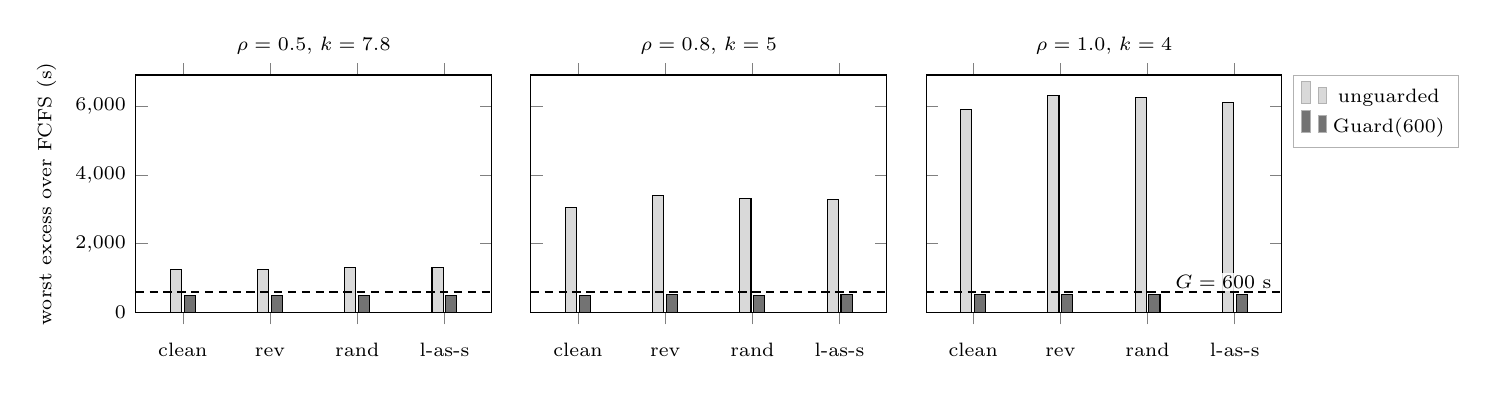
\begin{tikzpicture}[font=\footnotesize]
% RR-28: the x tick labels were rotated 40 degrees and cramped against each other in the
% narrow first panel, and the promise annotation sat at the left edge of that panel, where
% the y axis clipped it.  The panels are wider, the labels are set horizontally at
% \scriptsize (they are short enough), and the annotation moved into the third panel.
\pgfplotsset{
  excaxis/.style={
    width=6.1cm, height=4.6cm, ybar=1pt, bar width=4pt,
    symbolic x coords={clean,rev,rand,l-as-s}, xtick=data,
    ymin=0, ymax=6900, enlarge x limits=0.18,
    tick label style={font=\scriptsize}, label style={font=\scriptsize},
    title style={font=\scriptsize, yshift=-2pt},
    % text height/depth fixed so that the four labels share a baseline: with the default
    % anchor=north the box height follows the ascenders and "rev" would ride higher.
    x tick label style={anchor=north, yshift=-1pt, text height=1.6ex, text depth=0.45ex},
  },
}
\begin{axis}[excaxis, ylabel={worst excess over FCFS (s)},
             title={$\rho = 0.5$, $k = 7.8$}, name=q1]
  \addplot[fill=black!15] coordinates {(clean,1241.4) (rev,1240.1) (rand,1307.7) (l-as-s,1305.8)};
  \addplot[fill=black!55] coordinates {(clean,492.2) (rev,497.1) (rand,489.9) (l-as-s,497.1)};
  \draw[densely dashed] ({rel axis cs:0,0}|-{axis cs:clean,600}) -- ({rel axis cs:1,0}|-{axis cs:clean,600});
\end{axis}
\begin{axis}[excaxis, title={$\rho = 0.8$, $k = 5$}, yticklabels={},
             at={(q1.east)}, anchor=west, xshift=5mm, name=q2]
  \addplot[fill=black!15] coordinates {(clean,3044.5) (rev,3387.9) (rand,3319.4) (l-as-s,3292.0)};
  \addplot[fill=black!55] coordinates {(clean,507.8) (rev,513.5) (rand,504.5) (l-as-s,516.1)};
  \draw[densely dashed] ({rel axis cs:0,0}|-{axis cs:clean,600}) -- ({rel axis cs:1,0}|-{axis cs:clean,600});
\end{axis}
\begin{axis}[excaxis, title={$\rho = 1.0$, $k = 4$}, yticklabels={},
             at={(q2.east)}, anchor=west, xshift=5mm,
             legend style={font=\scriptsize, at={(1.03,1.0)}, anchor=north west,
                           draw=black!30, row sep=-1pt}]
  \addplot[fill=black!15] coordinates {(clean,5904.5) (rev,6295.7) (rand,6235.5) (l-as-s,6107.8)};
  \addlegendentry{unguarded}
  \addplot[fill=black!55] coordinates {(clean,523.7) (rev,534.8) (rand,520.7) (l-as-s,534.7)};
  \addlegendentry{Guard(600)}
  \draw[densely dashed] ({rel axis cs:0,0}|-{axis cs:clean,600}) -- ({rel axis cs:1,0}|-{axis cs:clean,600});
  \node[anchor=south east, font=\scriptsize, fill=white, fill opacity=0.85,
        text opacity=1, inner sep=1pt]
       at ({rel axis cs:0.98,0}|-{axis cs:clean,600}) {$G = 600$ s};
\end{axis}
\end{tikzpicture}}
\caption{Original-score reference and its corrupted-score controls. The worst single job, with and without the guard, under the
expected-cost score (``clean'') and the three corrupted scores of
Table~\ref{tab:s_adv}: reversed (rev), random (rand) and truly-longest-called-shortest
(l-as-s). The dashed line is the promise $G = \devnum{600}$ s. Sources: the clean
pair is the block header and the Guard($\devnum{600}$) row of
Table~4 of the manuscript; the three corrupted pairs are the ``Max excess'' columns
of Table~\ref{tab:s_adv}. The unguarded bar grows with load and with corruption;
the guarded bar does not, which is the content of Theorem~\ref*{M-thm:guard} of the manuscript and
not a property of the trace.}
\label{fig:excess}
\end{figure}


\subsection{The Bounds on the Traces}
\label{sec:exp_bound}

Every guarded run asserts the per-job bound of Section~\ref{sec:theory} for each job
separately, inside the simulation rather than afterwards on summary statistics. Across the
\devnum{315} policy-by-cell runs reported here, that is \devnum{5{,}554{,}949{,}400} per-job
checks with \devnum{0} violations, and the single-server configuration adds \devnum{21} runs and
\devnum{67{,}396{,}287} checks, also with \devnum{0} violations. An independently written
simulator, which shares no code with ours, reproduces the runs job for job on
\devnum{17{,}634{,}760} jobs and \devnum{22} policies with \devnum{0} differing jobs, and asserts
the same bounds on its own waiting times over \devnum{5.7} billion checks with \devnum{0}
violations; that cross-check was run against the earlier development pipeline, whose dispatch
sequence the package reproduces.

The ratio of the realised worst excess to the bound falls as $k$ grows. It reaches
\devnum{0.9950} at $k = 1$, \devnum{0.9311} at $k = 4$, \devnum{0.9219} at $k = 5$,
\devnum{0.8975} at $k = 7$ and \devnum{0.8850} at $k = 8$. This is a statement about these traces and not about
the constant: Section~\ref{sec:theory} shows $(3-2/k)L$ to be the exact supremum at every $k$,
but the family that approaches it is a geometric cascade that needs hundreds of jobs arranged
against the wrapper, and nothing in a replayed workload arranges them. The
finite-skip bound, by contrast, is attained exactly on small instances, at a ratio of
\devnum{1.0000}.

\paragraph{The identity, measured job by job.}
The net-overtake identity had been attacked on small synthetic instances but never measured on
the trace this paper runs on, so we measured it. Table~\ref{tab:resid} reports the residual
$D_i = k(W_P[i] - W_{\mathrm{FCFS}}[i]) - (\mathrm{In}_i - \mathrm{Out}_i)$ on overlay~0 at
the three load levels, under SPJF-E, Guard($\devnum{600}$) and the reversed score, with FCFS
on the same input as the reference schedule in every cell. Recovering $\mathrm{In}_i$ and
$\mathrm{Out}_i$ needs the dispatch sequence, which the guard kernel does not expose, so the
kernel and the independent reference simulator were each copied verbatim and given recorders
that add no branch and no state update; the two agree on the dispatch sequence of every job of
\devnum{3{,}000} random instances, the recording kernel reproduces the production kernel's
waits element for element inside every cell, and $\mathrm{In}_i$ and $\mathrm{Out}_i$ are
carried in exact integer microseconds, the currency the guard itself meters.

Theorem~\ref{thm:identity} is asserted on every job of every cell: \devnum{0} violations over
\devnum{1{,}428{,}415{,}560} job-checks, the \devnum{27} policies of this overlay at the three
loads, of which Table~\ref{tab:resid} prints nine. The residual stays far from its ceiling. The
largest $|D_i|$ among the printed cells is \devnum{6.788}$L$, at $k = \devnum{8}$, where the
bound $2(k-1)L$ is \devnum{14}$L$, and across the nine cells the maximum sits between
\devnum{0.485} and \devnum{0.514} of the bound, which is about $(k-1)L$; over all
\devnum{81} cells it never exceeds \devnum{0.517}. That is where a search that does not
build the cascade of Theorem~\ref{thm:tight1} stops, so the measurement says the workload does
not attain the constant, not that the constant is loose. Same-phase bookkeeping, the mechanism
behind the degenerate extremal instances of Remark~\ref{rem:directions}, accounts for at most
\devnum{0.36\%} of the total $\mathrm{In}$ in any cell, so the executed-work convention would
not change the picture here. The net-overtake term carries the per-job excess almost entirely:
$(\mathrm{In}_i - \mathrm{Out}_i)/k$ explains $R^2 = \devnum{0.983}$ to \devnum{0.9996} of the
variance of $W_P[i] - W_{\mathrm{FCFS}}[i]$, with a worst per-job error of \devnum{44.9} to
\devnum{50.9} s where the theorem permits $(2-2/k)L$, that is \devnum{90} s at $k = 4$ and
\devnum{105} s at $k = 8$. This is one overlay of development data, and the residual is a
property of a schedule rather than a statistic, so no interval is attached to it.

\begin{table}[htbp]
\centering
\caption{The residual $D_i$ of Theorem~\ref{thm:identity} on overlay~0,
\devnum{17{,}634{,}760} jobs per cell. Ratio is $\max|D_i|$ over the bound $2(k-1)L$,
which is \devnum{14}$L$, \devnum{8}$L$ and \devnum{6}$L$ at the three loads;
$R^2$ and the worst error are for $(\mathrm{In}_i - \mathrm{Out}_i)/k$
against the realised excess over FCFS.}
\label{tab:resid}
\small
\setlength{\tabcolsep}{3pt}
\begin{tabular}{llrrrrr}
\toprule
Load & Policy & $\max|D_i|/L$ & Ratio & $D_i = 0$ & $R^2$ & worst err.\ (s) \\
\midrule
$\rho = \devnum{0.5}$, $k = \devnum{8}$
 & SPJF-E              & \devnum{6.788} & \devnum{0.485} & \devnum{95.6\%} & \devnum{0.985} & \devnum{50.9} \\
 & Guard($\devnum{600}$) & \devnum{6.788} & \devnum{0.485} & \devnum{95.6\%} & \devnum{0.983} & \devnum{50.9} \\
 & Reversed score      & \devnum{6.788} & \devnum{0.485} & \devnum{95.6\%} & \devnum{0.996} & \devnum{50.9} \\
\midrule
$\rho = \devnum{0.8}$, $k = \devnum{5}$
 & SPJF-E              & \devnum{3.922} & \devnum{0.490} & \devnum{87.2\%} & \devnum{0.996} & \devnum{47.1} \\
 & Guard($\devnum{600}$) & \devnum{3.922} & \devnum{0.490} & \devnum{87.2\%} & \devnum{0.995} & \devnum{47.1} \\
 & Reversed score      & \devnum{3.881} & \devnum{0.485} & \devnum{87.5\%} & \devnum{0.999} & \devnum{46.6} \\
\midrule
$\rho = \devnum{1.0}$, $k = \devnum{4}$
 & SPJF-E              & \devnum{3.082} & \devnum{0.514} & \devnum{81.1\%} & \devnum{0.998} & \devnum{46.2} \\
 & Guard($\devnum{600}$) & \devnum{3.082} & \devnum{0.514} & \devnum{81.1\%} & \devnum{0.998} & \devnum{46.2} \\
 & Reversed score      & \devnum{2.994} & \devnum{0.499} & \devnum{81.7\%} & \devnum{1.000} & \devnum{44.9} \\
\bottomrule
\end{tabular}
\end{table}
% Source of Table~\ref{tab:resid}: outputs/paper_tables/tab_resid.tex, produced by
%   `python scripts/emit_paper_tables.py` (see GENERATED.md), from
%   outputs/dev_tables/identity_residuals.csv, rows overlay = 0, levels 0/1/2, policies
%   SPJF-E / Guard(600) / SPJF-reversed; columns max_abs_residual_L, ratio_to_bound,
%   share_residual_zero, r2_net_over_k, max_abs_error_s.  The load labels are the paper's
%   (rho = 0.5 / 0.8 / 1.0); the package prints the level index there.  The 1,428,415,560
%   job-checks and the 0.518 worst ratio are all 81 rows of the same file (27 policies x 3
%   loads x 17,634,760 jobs), column violations summing to 0.
%   The same-phase share of the paragraph above has no column in the package's residual file
%   and is quoted from prechecks/identity_residuals/out_SUMMARY.txt section 4
%   (samephase_share_sumIn), the earlier measurement of the same quantity on the same overlay.
%   The tool validation (3,000 random instances, sequence agreement with the independent
%   reference simulator, wait agreement with the production kernel) is section 1 of that file
%   and out_validate.txt.
% Source of Section~\ref{sec:exp_bound}: outputs/dev_tables/bound_checks.csv (315 rows,
%   jobs_checked summing to 5,554,949,400, violations 0, column used_over_allowed with maxima
%   0.9311 at k = 4, 0.9219 at k = 5, 0.8975 at k = 7 and 0.8850 at k = 8) and
%   outputs/dev_tables/k1/bound_checks.csv (21 rows, 67,396,287 checks, worst used/allowed
%   0.9950).  The independent simulator figures are prechecks/main_v3_verify/out_VERDICT.txt,
%   C2 and the "MAY" list, and prechecks/main_v3/out_main_v31.txt section 10 (finite-skip
%   used/allowed 1.0000); they verify the earlier pipeline, not the package.

\subsection{A Single Server}
\label{sec:exp_k1}

At $k = 1$ the additive constant $(3 - 2/k)L$ is exactly $L$, the identity of
Section~\ref{sec:theory} holds with no error term, and the separation between budget shapes is
largest (Table~\ref{tab:k1}). Guard($\devnum{600}$) and Fixed($\devnum{600}$) are
statistically indistinguishable on the gap closed and differ by a factor of \devnum{3.41} in
harm; the corresponding factors are \devnum{3.01} at $G = \devnum{300}$ s and \devnum{12.18} at
$G = \devnum{1200}$ s. The realised excess reaches \devnum{595.5} s against the promised
\devnum{600} s, and under the worst corrupted score \devnum{597.0} s, so at one server the
promise is close to being spent.

The single-server configuration also shows the cost of choosing a shape on one set of cells.
The parameters were selected on the \devnum{15} multi-server validation cells, and $k = 1$ is
not among them. At $G = \devnum{300}$ and $\devnum{600}$ s the joint winner transfers: it closes
\devnum{0.746} and \devnum{0.854} of the gap, against \devnum{0.543} and \devnum{0.791} for the
constant shape. At $G = \devnum{1200}$ s it does not: the queue-length shape that wins the
joint comparison on the multi-server cells closes \devnum{0.701} here, while the age-relative
shape closes \devnum{0.895} and the constant shape \devnum{0.865}. We report the number the
pre-stated rule produces and do not re-tune it on this cell; Section~\ref{sec:limits} states
what it means.

\begin{table}[htbp]
\centering
\caption{Single server, busy-hour $\rho = \devnum{0.80}$, \devnum{3{,}209{,}347} jobs. Waits and
excesses in seconds. The parameters are the ones the rule selected on the multi-server
validation cells; this configuration is not among them.}
\label{tab:k1}
\small
\setlength{\tabcolsep}{3pt}
\begin{tabular}{lrrlrrr}
\toprule
Policy & Promise & p99$_{\mathrm{dl}}$ & Gap closed & Max exc. & Harm & Fired (\%) \\
\midrule
FCFS                         & ---           & \devnum{221.27} & \devnum{0.000} & \devnum{0.0} & \devnum{0.0} & \devnum{100.00} \\
SJF on true sizes            & ---           & \devnum{45.32} & \devnum{1.000} & \devnum{2{,}054.5} & \devnum{777.9} & \devnum{0.00} \\
SPJF-E                       & ---           & \devnum{60.91} & \devnum{0.911 [0.854, 0.933]} & \devnum{2{,}520.3} & \devnum{656.4} & \devnum{0.00} \\
Guard($\devnum{300}$)        & \devnum{300} & \devnum{89.96} & \devnum{0.746 [0.571, 0.829]} & \devnum{297.9} & \devnum{81.8} & \devnum{8.17} \\
Guard-fixed($\devnum{300}$)  & \devnum{300} & \devnum{125.68} & \devnum{0.543 [0.207, 0.718]} & \devnum{140.3} & \devnum{119.5} & \devnum{17.09} \\
Guard-age($\devnum{300}$)    & \devnum{300} & \devnum{89.96} & \devnum{0.746 [0.571, 0.829]} & \devnum{297.9} & \devnum{81.8} & \devnum{8.17} \\
Guard-queue($\devnum{300}$)  & \devnum{300} & \devnum{105.15} & \devnum{0.660 [0.532, 0.715]} & \devnum{297.9} & \devnum{53.9} & \devnum{29.15} \\
Fixed($\devnum{300}$)        & \devnum{300} & \devnum{83.18} & \devnum{0.785 [0.584, 0.865]} & \devnum{297.9} & \devnum{246.3} & \devnum{6.33} \\
Skip($\devnum{300}$), $N=5$  & \devnum{300} & \devnum{220.39} & \devnum{0.005 [-0.002, 0.019]} & \devnum{95.1} & \devnum{81.8} & \devnum{73.17} \\
Guard($\devnum{600}$)        & \devnum{600} & \devnum{71.07} & \devnum{0.854 [0.780, 0.895]} & \devnum{595.5} & \devnum{165.5} & \devnum{2.53} \\
Guard-fixed($\devnum{600}$)  & \devnum{600} & \devnum{82.10} & \devnum{0.791 [0.602, 0.868]} & \devnum{303.0} & \devnum{246.3} & \devnum{6.16} \\
Guard-age($\devnum{600}$)    & \devnum{600} & \devnum{71.07} & \devnum{0.854 [0.780, 0.895]} & \devnum{595.5} & \devnum{165.5} & \devnum{2.53} \\
Guard-queue($\devnum{600}$)  & \devnum{600} & \devnum{91.52} & \devnum{0.737 [0.640, 0.812]} & \devnum{582.0} & \devnum{81.8} & \devnum{3.43} \\
Fixed($\devnum{600}$)        & \devnum{600} & \devnum{68.48} & \devnum{0.868 [0.783, 0.906]} & \devnum{593.4} & \devnum{563.6} & \devnum{2.29} \\
Skip($\devnum{600}$), $N=10$ & \devnum{600} & \devnum{219.89} & \devnum{0.008 [-0.004, 0.037]} & \devnum{100.9} & \devnum{83.2} & \devnum{66.98} \\
Guard($\devnum{1200}$)       & \devnum{1200} & \devnum{98.00} & \devnum{0.701 [0.640, 0.742]} & \devnum{1{,}157.4} & \devnum{53.9} & \devnum{26.15} \\
Guard-fixed($\devnum{1200}$) & \devnum{1200} & \devnum{69.03} & \devnum{0.865 [0.789, 0.905]} & \devnum{564.2} & \devnum{509.3} & \devnum{2.57} \\
Guard-age($\devnum{1200}$)   & \devnum{1200} & \devnum{63.80} & \devnum{0.895 [0.835, 0.920]} & \devnum{1{,}182.3} & \devnum{366.4} & \devnum{0.68} \\
Guard-queue($\devnum{1200}$) & \devnum{1200} & \devnum{98.00} & \devnum{0.701 [0.640, 0.742]} & \devnum{1{,}157.4} & \devnum{53.9} & \devnum{26.15} \\
Fixed($\devnum{1200}$)       & \devnum{1200} & \devnum{63.19} & \devnum{0.898 [0.837, 0.923]} & \devnum{1{,}180.4} & \devnum{656.4} & \devnum{0.45} \\
Skip($\devnum{1200}$), $N=20$ & \devnum{1200} & \devnum{217.64} & \devnum{0.021 [-0.008, 0.084]} & \devnum{168.0} & \devnum{97.7} & \devnum{58.67} \\
\bottomrule
\end{tabular}
\end{table}
% Source of Table~\ref{tab:k1}: outputs/paper_tables/tab_k1.tex, produced by
%   `python scripts/emit_paper_tables.py` (see GENERATED.md), from
%   outputs/dev_tables/k1/main_table.csv; columns p99_dl_s, gap_closed with gap_closed_lo/hi,
%   max_excess_s, harm_s, fired_pct, and the promise G.  The harm ratios 3.01 / 3.41 / 12.18 in
%   the text are Fixed(G) harm over Guard(G) harm from the same rows.  The adversarial excess
%   597.0 s is the Guard(600)-top1short row of the same file, column max_excess_s.  The two
%   third-decimal double-rounding errors the verifier found in the previous version of this
%   table (item G2: Fixed(600) gap upper bound, and the promise-90 "Fixed, admitted" row) are
%   gone with the rows and the rounding: every figure here is printed once from the package's
%   own full-precision column.

\subsection{Other Platforms}
\label{sec:exp_cross}

Table~\ref{tab:cross} places the main trace beside five others under one format. The first three
columns describe the workload, the next two what ranking by prediction does to it without a
guard, and the last two what the guard keeps and what it caps at a promise of five job-limits.
Excesses are expressed in units of the per-job limit $L$, which is the unit the guarantee is
written in.

% Wider than the MDPI text block: set across the full page with the template's
% adjustwidth/\extralength mechanism.
\begin{table}[htbp]
\begin{adjustwidth}{-\extralength}{0cm}
\centering
\caption{The same method on six workloads. Tail share is the fraction of executed work carried
by the longest \devnum{1\%} of jobs; AUROC is for the heavy class from arrival-time information;
excesses are in units of the per-job limit $L$ of that trace.}
\label{tab:cross}
\small
\setlength{\tabcolsep}{3pt}
\begin{tabular}{lcccccc}
\toprule
 & Tail & & FCFS & Gap & Unguarded & Guard at $G \approx \devnum{5}L$ \\
Trace and load & share & AUROC & p99$/L$ & SPJF-E & max exc. & gap kept / max exc. \\
\midrule
CodeBench, busy-hour $\rho = \devnum{1.06}$ & \devnum{0.375} & \devnum{0.928} & \devnum{4.39} & \devnum{0.916} & \devnum{98.4}$L$ & \devnum{0.478} / \devnum{3.82}$L$ \\
ACcoding, drawn arrivals, $\rho = \devnum{0.8}$ & \devnum{0.122} & \devnum{0.927} & \devnum{0.021} & \devnum{0.980} & \devnum{20}$L$ & \devnum{0.974} / \devnum{2.21}$L$\textsuperscript{a} \\
Serverless, busy-hour $\rho = \devnum{1.0}$ & \devnum{0.443} & \devnum{0.985} & \devnum{4.22} & \devnum{0.858} & \devnum{10.07}$L$ & \devnum{0.710} / \devnum{2.52}$L$ \\
CI pool A, $k_{\mathrm{eff}} = \devnum{156}$ of \devnum{173} & \devnum{0.034} & \devnum{0.651} & \devnum{1.78} & n/a\textsuperscript{b} & \devnum{11.53}$L$ & \devnum{0.735}\textsuperscript{b} / \devnum{2.64}$L$ \\
CI pool B, $k_{\mathrm{eff}} = \devnum{96}$ of \devnum{105} & \devnum{0.052} & \devnum{0.997} & \devnum{0.373} & \devnum{0.958} & \devnum{0.34}$L$ & \devnum{0.958} / \devnum{0.34}$L$ \\
Compute farm, window $\rho = \devnum{0.95}$ & \devnum{0.372} & \devnum{0.890} & \devnum{0.136} & \devnum{$-4.111$} & \devnum{0.85}$L$ & \devnum{$-4.346$} / \devnum{0.83}$L$ \\
\bottomrule
\end{tabular}

\vspace{2pt}
\begin{minipage}{\fulllength}
\footnotesize
\textsuperscript{a} ACcoding arrival instants are drawn, not recorded, so every scheduling figure
in this row is a statement about the ordering mechanism and not about waiting on that platform;
its budgets were set at fixed multiples of $L$ rather than from a promise, and the entry shown
is the largest one tested, $B = \devnum{10}L$.
\textsuperscript{b} On CI pool A, SJF is itself worse than FCFS at the p99, so the p99 gap has
no usable denominator; the guard entry is the mean-wait gap.
\textsuperscript{c} The CI capacities are fitted, not recorded, and the two scheduling
columns and the FCFS p99 of these rows exist only at the whole-window fit
($k_{\mathrm{eff}} = \devnum{156}$ of \devnum{173} and \devnum{96} of \devnum{105}), so they
are printed at it. What supports them is the held-out refit of Section~\ref{sec:data}, which
recovers the same capacity to within a few machines on chronological splits of each window and
reproduces the recorded waits on the untouched part, with the p90 the one quantile that does
not survive. The tail share and the AUROC do not depend on the capacity.
\end{minipage}
\end{adjustwidth}
\end{table}
% Source of Table~\ref{tab:cross}:
%   CodeBench row: tail share from prechecks/codebench_audit/out_tail_and_counts.txt via
%     Table~\ref{tab:tails}; AUROC from prechecks/codebench_service_v2/out_service_v2.txt
%     SUMMARY 1 (config ires0, train core, M4); FCFS p99/L from
%     prechecks/cross_domain/out_cross_domain_table.txt section C, row
%     "CodeBench busy-hour rho=1.06"; the gap, the unguarded max excess (5,904.5 s / 60 = 98.4 L)
%     and the guard entry (Guard(300): gap 0.478, max excess 229.1 s = 3.82 L) from
%     Table~\ref{tab:guard}, level rho = 1.0, which supersedes the CodeBench rows
%     of the cross-domain file.
%   ACcoding, Serverless and Compute farm rows: prechecks/cross_domain/out_cross_domain_table.txt,
%     sections A (top1% work), B (AUROC), C (FCFS p99/L, gap SPJF, SPJF max excess in L) and D
%     (guard 5 L: gap p99 and max excess in L); the ACcoding guard entry is instead
%     prechecks/accoding_v2/out_accoding_v2.txt, block "sim poisson_rho0.8_main", row
%     GUARD-M4-B305, columns gain_p99 (0.974) and max_exces (67.5 s = 2.21 L).
%   CI pool rows: prechecks/firefox_ci/out_SUMMARY.txt, section A (top 1% work share), section C
%     (ALL/log AUROC), section D (FCFS p99/L', gap SPJF, SPJF max excess, and the G = 5 L' guard
%     rows: gap mean 0.7351 and max excess 2.6441 L' for pool A, gap p99 0.9576 and max excess
%     0.3384 L' for pool B), section E (the p99/L' ratios).  Section D exists only at the
%     whole-window fitted capacities k_eff = 156 (pool A) and 96 (pool B), which is why the two
%     scheduling columns and the FCFS p99/L of those rows keep the whole-window fit; footnote c
%     says so.  The held-out figures in footnote c are
%     prechecks/firefox_ci_holdout/out_SUMMARY.txt section A (k_eff step-1 grid per split:
%     osx 155/155/157 of 173, talos 96/92 of 105) and section F (held-out mean 0.90-1.14,
%     p99 0.86-1.16, p90 0.81-1.21); the same rows are in holdout.csv.  The row labels now name
%     the fitted capacity instead of calling it "recorded capacity", which it was not.

Two conditions decide whether the method is worth applying, and each has a trace here that fails
it. The first is that the per-job limit $L$ must be small next to the waits the operator cares
about. The smallest promise the guarantee family can express is $(3 - 2/k)L$, close to
\devnum{3}$L$, so a workload whose FCFS p99 wait is below that ratio cannot be given a promise
finer than the wait it is about. The ratio is \devnum{4.39} on CodeBench and \devnum{4.22} on the
serverless trace, \devnum{1.78} on CI pool~A and \devnum{0.136} on the compute farm, whose jobs
run for days: in that window its FCFS p99 wait is \devnum{18.7} h against a per-job limit of
\devnum{493{,}857} s, or \devnum{5.7} days. The second is that costs must be heavy-tailed. On the
CI pools the longest \devnum{1\%} of jobs carry \devnum{3.4\%} and \devnum{5.2\%} of the work,
and SJF makes the p99 wait worse than FCFS on three of the four windows we ran, so there is no
p99 benefit to transmit and the gap statistic has no denominator. Where both conditions hold, the
guard keeps \devnum{0.48} to \devnum{0.71} of the gap and caps the observed excess at
\devnum{2.5} to \devnum{3.8}$L$ at a promise of \devnum{5}$L$.

\subsection{Sensitivities}
\label{sec:exp_sens}

Five variations of the trace construction and of the availability protocol were run through the
same pipeline (Table~\ref{tab:sens}). None of them reverses the result and the two that move it
move it upwards, so the primary pool is the conservative choice: adding the term whose busiest
hour is dominated by runs that outlived their container raises the gap, and the opposite reading
of the timestamp, in which the stamp is receipt rather than completion, gives
\devnum{0.926} against \devnum{0.895}. Merging or dropping the groups of runs by one user that
end in the same second moves the gap closed by \devnum{0.017} and \devnum{0.003} at full load,
so the stretching between concurrent runs of one user is not what produces the result, and
delaying the visibility of a completed job's outcome costs prediction quality and not much of
it (Section~\ref{sec:prediction}). The guard's benefit is the quantity most sensitive to the
construction, ranging from \devnum{0.442} to \devnum{0.843} of the gap at a fixed budget of
\devnum{600} s at full load.

\begin{table}[htbp]
\centering
\caption{Trace-construction sensitivities at busy-hour $\rho = \devnum{1.0}$, three overlays,
fraction of the deadline-window gap closed.}
\label{tab:sens}
\small
\setlength{\tabcolsep}{4pt}
\begin{tabular}{lcrcc}
\toprule
Variant & $k$ & FCFS p99$_{\mathrm{dl}}$ & Unguarded & Guard, budget \devnum{600} s \\
\midrule
Primary pool (overlays 0--2) & \devnum{4.000} & --- & \devnum{0.895 [0.864, 0.916]} & \devnum{0.442 [0.345, 0.631]} \\
Earlier term added           & \devnum{4.667} & \devnum{95.41}  & \devnum{0.945 [0.885, 0.965]} & \devnum{0.843 [0.715, 0.880]} \\
Co-ending runs merged        & \devnum{4.000} & \devnum{228.19} & \devnum{0.912 [0.892, 0.924]} & \devnum{0.603 [0.445, 0.740]} \\
Co-ending runs dropped       & \devnum{4.000} & \devnum{209.30} & \devnum{0.898 [0.879, 0.914]} & \devnum{0.608 [0.471, 0.753]} \\
Opposite timestamp reading   & \devnum{4.000} & \devnum{268.75} & \devnum{0.926 [0.904, 0.939]} & \devnum{0.545 [0.422, 0.699]} \\
\bottomrule
\end{tabular}
\end{table}
% Source of Table~\ref{tab:sens}: prechecks/codebench_service_v2/out_service_v2.txt, SUMMARY 5,
%   the four blocks "pool19 / sbatch / sdrop / isub0 (3 reps), target rho 1.0"; columns k,
%   p99_dl (FCFS row), and the variant's own gain_p99_dl for rows SPJF-M4 and GUARD-M4-B600.
%   The "Primary pool" row is the "primary(0-2) gain_p99_dl" column of the same blocks, which
%   is why it carries no FCFS p99 of its own.  The delta figures in the text are SUMMARY 1 of
%   the same file, table "auroc, all test rows", row (core, M4), columns ires0, ires600, isub0,
%   isub60, isub600, isub3600.

Two further limits of these runs are stated where they belong. The intervals resample whole
weeks of one overlay construction, so they cover time and not the choice of terms, and five
overlays are five week-shifts of the same \devnum{40} class-terms rather than five platforms.
The runs compare scheduling policies on a common set of enqueue instants and do not charge the
cost of computing features and predictions; Section~\ref{sec:prediction} measures that cost
separately, and Section~\ref{sec:limits} states what it would take to claim an end-to-end
result.
